
\chapter{}
\label{chap:guide}

\section{预脉冲与预等离子体}
\begin{figure}[!htbp]
  \centering
  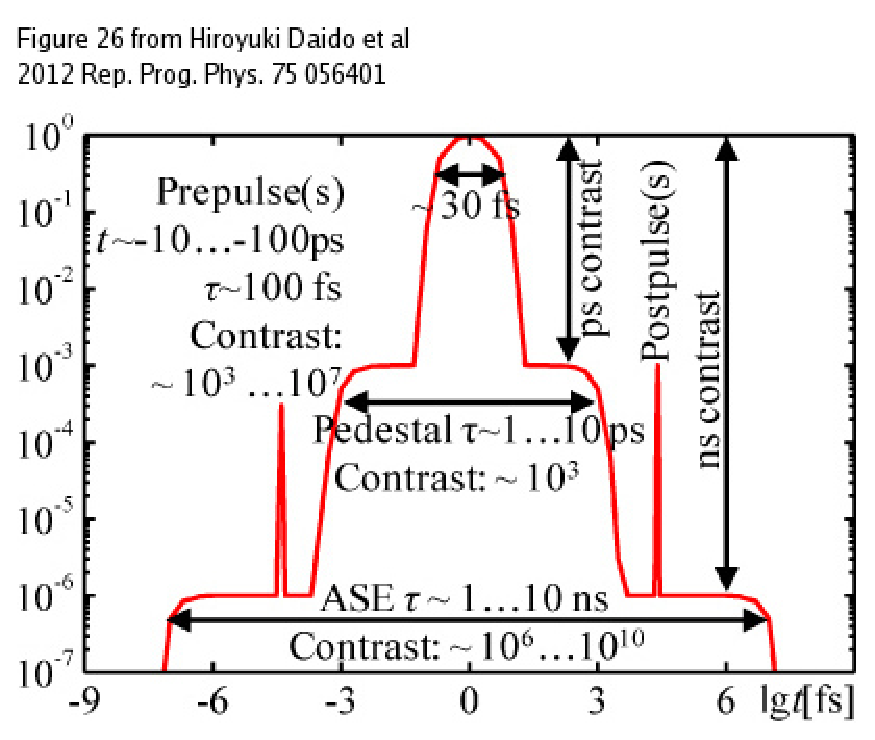
\includegraphics[width=\MyFactor\textwidth]{Img/prepulse2012.eps}
  \caption{激光脉冲示意图}
  \label{fig:prepulse2012}
\end{figure}

实际上,在实验中激光脉冲并不是只有一个主脉冲,其时间结构如图\ref{fig:prepulse2012}所
示。在峰值强度之前的激光可以统称为预脉冲,从前到后依次是:1、Replica:
位于主脉冲前7ns到十几ns的位置,是相干的短脉冲,也可称为fs预脉冲。2、ASE
(自发放大辐射):位于主脉冲之前几个ns的位置,时间宽度为ns量级。ASE是
非相干的光。3、Pedestal:位于主脉冲前100ps内。从产生原因来看:fs预脉冲
是再生放大器在选单或倒空的过程中,由于高压电脉冲的上升沿不够陡峭,或者
普克尔盒对高压电脉冲的响应不够快,响应时间太长,造成普克尔盒消光比不够
高,在主脉冲的前后有几个间隔为7ns左右(由再生腔长决定)的激光脉冲从再
生腔中输出并在后面的主放大器中得到进一步的放大,并在经过压缩器压缩后成为
脉宽与主激光基本相同的fs脉冲。ASE(自发放大辐射)主要来源于预放大器和主
放大器晶体内的自发辐射。由于钛宝石晶体的增益较高,增益介质中产生的自发辐
射会在放大链中也得到放大,从而形成放大的自发辐射。它位于主脉冲前几个ns的
位置,持续时间为ns量级。最后由于振荡器内的杂散光或者漏光,以及压缩光栅对
光脉冲的不完全压缩,会在主脉冲前100ps内形成一个平台区Pedestal。


在激光脉冲作用的过程中,其物理图像如此:在主脉冲之前,ASE和预脉冲已经把
靶材前表面加热电离,形成等离子。前表面的等离子体向真空膨胀,在靶前形成
预等离子体。与此同时,激光在靶面产生Mbar量级的压强,形成冲击波向靶内传
输。如果靶材较薄,在主脉冲到来前冲击波传播到靶的后表面,将后表面破坏造
成其向真空膨胀,靶后与真空不再有锐利的分界面,形成密度标长较长的区域,
降低加速效率,但是厚靶又不利于TNSA鞘层加速。因此靶材厚度存在一个最佳值,
既能获得较高的鞘层加速效率,又将冲击波的影响降到最低。显然,这个最佳值
将随冲击波的强度变化。在实验中预脉冲和ASE同时存在,两者均能在靶前产生预等离子体,并
在靶内形成冲击波,从而改变靶的密度分布。


我们对ASE和fs预脉冲产生的作用进行理论分析。
首先是靶材的前表面被离化后,等离子体向真空自由膨胀的过程。根据Mora
等人的工作\cite{mora2003plasma,mora2005thin},假设等离子体的自由膨胀是等温过程后,通过解析计算得
到等离子体的波前速度公式为:
\begin{equation}
\label{eqn:waveFrontVelocity}
v_{max}=2 c_s ln(\tau + \sqrt{{\tau}^2+1})
\end{equation}     
其中$c_s=(Z k_B T_e / m_i)^{1/2}$为离子声速度,$T_e=m_e c^2 \sqrt{1+\frac{I {\lambda}^2}{{1.37} \times {10}^{18} W/cm^2 \cdot \mu m^2}}$ 是电子能量\cite{kruer1985j},$\tau={\omega}_{pi} t_{acc}/(2e)^{1/2}$为归一化加速时间, ${\omega}_{pi}=[(Z_i e^2 n_e)/(m_i {\epsilon}_0)]$,J. Fuchs \cite{fuchs2006laser} 通过对部分实验数据进行拟合得到离子加速的参考时间约为 $t_{acc} \approx 1.3 t_{laser}$。
fs预脉冲只在飞秒的脉冲时间与等离子相互作用,ASE却在
ns的时间内持续作用。因此ASE 对于前表面预等离子体的产生起到主导的作用。


其次需要计算预脉冲和ASE所产生的冲击波对靶后表面的影响。由于ASE是从
7ns逐渐增长至最大值(即所列数值),且其强度比fs预脉冲低一个量级,对靶
后的破坏远不如fs预脉冲,所以下面的主要讨论fs预脉冲的作用。由激光脉冲所
引起的冲击波压强为\cite{lindl1995development}:
\begin{equation}
\label{eqn:shockPressure}
P= \zeta I ^{2/3}
\end{equation}     

其中 P 是压强,以$P_a$为单位;I是激光光强,以$W/m^2$ 为单位;$\zeta$ 是材料常数,对于波长为0.8um的激光,Al靶和Cu靶可分别近似为 $J^{1/3} s^{2/3} m^{5/3} $和
$0.75 J^{1/3} s^{2/3} m^{5/3} $
\cite{swift2004shock}。对于受到冲击波作用的靶材,因为初始时处于静止状态,
所以根据质量和动量守恒定律,冲击波波前的传播速度$v_s$ 和离子的速度$v_p$满足
\begin{equation}
\label{eqn:shockEquation1}
\rho_0 v_s = \rho (v_s - v_p)
\end{equation}     

\begin{equation}
\label{eqn:shockEquation2}
P= \rho_0 v_s  v_p
\end{equation}     

\begin{equation}
\label{eqn:shockEquation3}
v_s = c_0 + \alpha v_p
\end{equation}     

其中 $\rho_0$ 和$\rho$分别是靶材初始密度和被压缩后的密度, $c_0$ 是声速,$\alpha$与材料有
关的经验常数。Al靶$c_0=5.24 \mu m/ns$ , $\alpha=1.40$,Cu靶$c_0=3.94 \mu m/ns$,$\alpha=1.49$\cite{lundh2007influence}。利用\ref{eqn:shockEquation1,eqn:shockEquation2,eqn:shockEquation3}求解$v_s$,$v_p$得

\begin{equation}
\label{eqn:shockV}
v_s = \frac{c_0}{2} (\sqrt{1+x}+1)
\end{equation} 

\begin{equation}
\label{eqn:pressureV}
v_s = \frac{c_0}{2}(\sqrt{1+x}-1)
\end{equation} 


其中$x=(4 \alpha / {\rho}_0 {c_0}^2)P$ 。当冲击波到达靶后与真空的交界面后,冲击波压强变
为零,被压缩的靶的后表面开始以$2v_p$ 速度向真空膨胀,同时形成松弛波
(relaxation wave)以离子声速向靶内传播。当靶内压力下降到零之后,根据
靶后的最终物质状态可以分为两种情况。第一种情况是冲击波压强小于$1.2Mbar$
(相应的预脉冲强度为$5 \times {10}^{12}W/{cm}^2$ ),靶后物质低于气相点,靶与真空之间还
有明显的分界面;第二种情况是当冲击波压强大于2Mbar(相应的预脉冲强度为
${10}^{13}W/{cm}^2$ ),靶后被完全气化,形成大密度标长的等离子体,导致难以有效的
建立鞘层场\cite{batani2010effects}。

但是,如果ASE强度相当且远低于fs预脉冲,并且fs预脉
冲在ASE达到最大值前的几个ns就与靶相互作用,fs预脉冲对靶后表面的破坏作用
远大于ASE。




\section{预等离子体的数值计算}


我们关注的问题是, 对于目前相对论fs激光实验室条件下的,强度在$10^{12}-10^{15} W/cm^2$,脉冲周期在ps到ns量级的预脉冲,对于$\mu m$金属薄膜靶的作用。其中的存在且关注的重要物理过程有:激光的吸收,能量的传输,金属靶的离化,电子和离子的加热,靶前表面等离子体的膨胀,压力波向靶后的传播等。


辐射压流体力学程序MULTI是由R. Ramis 开发的,用于研究强激光与物质作用过程中流体力学过程,在研究预脉冲与金属靶作用领域有着一定的应用。其基本的构成是典型的流体力学程序结构:


\subsection{流体力学过程}
由质量、动量、以及能量守恒方程组成的流体运动方程
\begin{equation}
\label{eqn:massCon}
D_t \rho = - \rho \nabla \cdot \bf{v}
\end{equation} 

\begin{equation}
\label{eqn:momentumCon}
\rho D_t \bf{v} = - \nabla P - \bf{R}
\end{equation} 

\begin{equation}
\label{eqn:energyCon}
\rho D_t e = -P \nabla \cdot \bf{v} - \nabla \cdot \bf{q} -Q +S
\end{equation} 

其中, 密度$\rho$,速度$v$,压强$P$,辐射动量$R$,内能$e$,能量密度$Q$,能流$\bf{q}$,外部能量源$S$ 。


\subsection{激光的吸收}
对于我们关注的固体靶烧蚀问题中,外部能量源是非相对论激光脉冲,而激光的吸收耦合因子是一个初始设定的变量。建立在对于吸收机制明确的基础上,这种假设成立。然而激光强度增加之后,电子的异常加热机制(真空加热,共振加热,以及更高强度的 J x B 加热等)得到显著的增强,此时这种处理不再有效。对于强度低于 $10^18 W/cm^2$的非相对论激光脉冲,
其能量沉积主要发生在临界密度以下等离子体中,
入射光$I_{+}(x,t)$和发射光$I_{-}(x,t)$满足;
\begin{equation}
\label{eqn:incidentLaser}
\partial_x I_{+}= \kappa I_{+}
\end{equation} 

\begin{equation}
\label{eqn:reflectLaser}
\partial_x I_{-}= -\kappa I_{-}
\end{equation} 
其中$\kappa$是吸收耦合因子,
\begin{equation}
\label{eqn:Kappa}
\kappa =C \frac{1}{T^{3/2}} \bigl( \frac{\rho}{\rho_c}  \bigr) \frac{1}{\sqrt{1-\rho/ \rho_c}}
\end{equation} 
$\rho_c=n_c m_i / Z_i$是离子临界密度,$n_c$是电子临界密度,$m_i$和$Z_i$分别是离子质量和电量。
已知$I_-$和$I_+$,能量沉积项:
\begin{equation}
\label{eqn:energyDeposition}
S=\partial_x I_+ \partial_x I_-
\end{equation} 

\subsection{能量传输}
激光的吸收通过\ref{eqn:energyCon}耦合到流体方程中,
沉积在等离子体中的能量,主要通过电子传输,近稳态近似下,热流满足Spitzer公式:
\begin{equation}
\label{eqn:heatFlux}
q=-\bar{K} T^{5/2} {\partial}_x T
\end{equation} 
$\bar{K}$ 满足
\begin{equation}
\label{eqn:kBar}
\bar{K}=\frac{10.16 \epsilon \delta_t k^{7/2}}{\sqrt{m_e}e^4 Z_i log \Lambda}
\end{equation} 
且:
\begin{equation}
\label{eqn:heatFlux1}
\epsilon \delta_t \approx 0.095 \frac{Z_i+0.24}{1+0.24Z_i}
\end{equation} 

$k$ 是玻尔兹曼常熟,$m_e$ 和 $e$ 电子的质量与电量,$Z_i$是有效的离子带电量,$\Lambda$
是库仑对数。

但是对于较大的温度梯度,公式不再成立,通常算法是热流中引入如下变量:
\begin{equation}
\label{eqn:freeStream}
q_{fs}=-n_e k T (k T / m_e)^{1/2}
\end{equation} 
并通过差值的方法解决。





传输过程确定了能量的分布,传输过程完成后,通过状态方程的方法,更新温度,压强,辐射度等变量,MULTI使用的是SESAME库处理状态方程的求解。对于不同属性材料,使用表格的形式,对于状态方程离化处理。基本的变量为密度$\rho$和内能$e_i$, 其导出量: 温度$T(\rho, e_i)$,压强$P(\rho, e_i)$,平均电离度$\bar{Z}(\rho, e_i)$,辐射性$\epsilon_k(\rho, e_i)$(其中k表示不同的辐射频率)等。




在拉格朗日描述的基础上,通过流体力学基本方程及假设,以格点为单位,计算能量的吸收,由于状态方程得到温度压强等,更新速度,体积等。然后将拉格朗日坐标系转化为欧拉坐标系,但是变换后的变量在空间上不具有连续性,需要使用插值的方法对此进行修正。



其计算流程如下:
1 初始化过程,根据初始条件设定,以流体元为基本的单元,将质量m和 能量$E$,体积$V$,密度$\rho$,温度$T$,压强$P$等热力学变量及其导出变量,存贮到计算格中。而$\vec{p}$ $\vec{v}$ 存贮在计算格的顶点中,因此格子的大小是可以改变的,格子中的质量元是常量。

能量的沉积是由于电子的






以下的流体力学模拟基于北京大学强激光实验室,其参数如下:
激光激光主脉冲能量5J,脉冲的脉宽为30fs,焦斑半径5um,预脉冲对比度$10^{-9}$,预脉冲强度为$10^12W/cm^2$,时间尺度为1ns范围内。我们采用$\mu m$量级铝靶进行烧蚀,烧蚀过程中每10ps进行采样,包括电子的密度,压强,温度等最终得到的结果可以在相应的时间做出一维结果分析。计算过程采用100格点进行解析,同时采用100ns的时间分辨率。

\subsection{铝靶烧蚀}

作用中采用的材料为铝靶,其厚度在um量级,为激光加速试验中常用的材料。 采用multi1D2009程序对于烧蚀过程进行模拟,结果如下, 


其中图1 是密度的分布,颜色分别表示激光作用时间 的结果。激光在t=0时刻由左侧作用在等离子体上,激光能量沉积在靶中,可以假设有一个吸收面,而吸收面处由于温度梯度产生热压力,热压向左右两侧同时传播,左侧向真空中传播造成等离子体的膨胀,右侧的热压向靶内部传播形成高密度压力波前沿。在t=100ps时已经可以看到明显的压缩前沿了,而其位置正好对应于压力波前的位置,其速度可由上节中的理论进行估算。应该注意在t=500ps时压力波前沿已经完全至靶后,因此500ps之后的靶后表面结构已经明显被破坏了,而这对于鞘层加速是有害的,因此对于加速时应该尽量避免的。因此在光强10…12 时候,激光的脉冲宽度应该控制在500ps内部,否则预脉冲对于加速将起到负面的作用,这就解释了众多的离子加速试验中的结果都低于模拟中的预期结果了。总体的趋势,随着时间的增长,等离子体密度的膨胀距离更大,而且等离子体的标度也更大,密度的分布变得更加平缓,而预等离子体的分布主要集中在了临街密度的区域,因为激光的吸收主要在临界密度区域,压力波的前向传播对于等离子体的密度影响由自由膨胀模型所决定。




其次在图2中,我们得到了压强的分布,压强的位置对应于密度压缩前沿的位置,当压力波传到靶后,靶后被破坏,而且压力波瞬间减少。如图中对应于500ps的分布。靶后表面的变形对于加速是有害的,这一点已经有实验所验证,因此尽量避免。压力波在靶内部的传播速度由靶材料温度等决定,由于压力波的传播速度可以估计靶后被破坏的时间。而实际的实验中尽量减小预脉冲的时间尺度,从而排除由于靶后表面的破坏造成对加速负面效应。


同时图3中,我们得到了温度的分布情况,电子的加入集中在临界密度区域,这符合理论分析的结果。同时可以看出电子的加热在向前的方向。而向后的方向几乎没有高温电子的分布,因此后表面破坏不是电子的等离子体膨胀造成的,更多是由于压力波形成的如shock结果传播的结果。经过1ns的烧蚀作用,电子的温度最大值已经可以达到100KeV的量级,这这样的电子温度对于激光与等离子体作用中的不稳定性具有有很重要的意义。



\subsection{DLC烧蚀}

北京大学镀膜实验室中能够生产类金刚石薄膜靶(DLA),其最小厚度可以达到10nm,是用于激光光压RPA加速的重要材质。然而重要的问题在于,由于DLA很薄,激光预脉冲可以很轻易的将其气化,而无法满足RPA对于等离子体靶的基本要求。即便是对于fs量级的预脉冲,这样的影响也是相当地。因此,DLA烧蚀作用的研究是非常必要的过程。
同样也是基于现有的实验中的方案采用30fs的激光脉冲对于DLA进行烧蚀,研究再次过程中DLA靶的密度以及温度等演化过程。而研究的工具是multifs工具,同样是由Rafael. Ramis 开发的工具,其计算过程采用的模型不同于multi2009中的流体力学模型,而是采用了求解电磁场的方法,求解格点内部的状态方程,最终得到密度,温度,压强等宏观可测参量。再次不对其具体算法进行详细介绍。






此外,另一个应用在于对于碳纳米管的烧蚀的研究。彬建辉等提出了一种产生预等离子体的方法,是利用激光烧蚀间隔分布的碳纳米管,由于纳米管被烧蚀膨胀气化,最终形成的等离子体均匀且密度可能。因此对于碳纳米管烧蚀产生的等离子体的分布就是一个有意义的问题。

\subsection{结论}
